\documentclass[10pt,a4paper]{article}
\usepackage[utf8]{inputenc}
\usepackage[T1]{fontenc}
\usepackage[margin=2cm]{geometry}
\usepackage{graphicx}
\usepackage{booktabs}
\usepackage{amsmath}
\usepackage{subcaption}
\usepackage{xcolor}
\usepackage[hidelinks]{hyperref}
\usepackage{titlesec}
\titlespacing*{\section}{0pt}{6pt}{3pt}
\titlespacing*{\subsection}{0pt}{4pt}{2pt}
\setlength{\parskip}{2pt}
\setlength{\parindent}{0pt}
\graphicspath{{../analysis/out/}}

\newcommand{\TEAMMEMBERS}{Marco Reczuch \and David Birgel \and Jerome Engelbrecht}
\newcommand{\Ntrain}{29688}
\newcommand{\Ncal}{1924}
\newcommand{\Nval}{1124}
\newcommand{\Nkept}{29376}
\newcommand{\Ndup}{312}
\newcommand{\Nbad}{0}
\newcommand{\RealNonSquare}{4741}
\newcommand{\RealSquare}{146}
\newcommand{\AiSquare}{24489}
\newcommand{\Targetfpr}{0.15}
\newcommand{\ImgSize}{64}
\newcommand{\CnnParams}{430}
\newcommand{\BaseValFpr}{0.101}
\newcommand{\BaseValRecall}{0.699}
\newcommand{\BaseAugFpr}{0.262}
\newcommand{\BaseAugRecall}{0.474}
\newcommand{\CnnValFpr}{0.176}
\newcommand{\CnnValRecall}{0.802}
\newcommand{\CnnAugFpr}{0.225}
\newcommand{\CnnAugRecall}{0.664}
\newcommand{\AugValFpr}{0.181}
\newcommand{\AugValRecall}{0.756}
\newcommand{\AugAugFpr}{0.107}
\newcommand{\AugAugRecall}{0.618}
\newcommand{\OccCenterReal}{-0.094}
\newcommand{\OccBorderReal}{-0.053}
\newcommand{\OccCenterAi}{-0.056}
\newcommand{\OccBorderAi}{-0.017}
\newcommand{\RefSeconds}{479}
\newcommand{\TrainSeconds}{1640}
\newcommand{\TrainRatio}{3.43}


\title{\vspace{-1.5em}\textbf{AMLS SoSe 2026 — AI Image Detection}}
\author{\TEAMMEMBERS}
\date{\vspace{-1em}\today}

\begin{document}
\maketitle
\vspace{-1.5em}

\section{Introduction and Data}
Within this project, we have built a CPU dedicated pipeline capable of
classifying given images as being \emph{real} (0) or generated by AI models (1),
five generators (SD\,2.1, SDXL, SD\,3, DALL-E\,3, Midjourney) are combined into
class~1. The data that has been labelled ($\Ntrain$ train, $\Ncal$ calibration,
$\Nval$ validation images, plus augmented counterparts) is made of JPEG images.
The unlabelled \texttt{predict/} split score gets calculated at the inference
step. The pipeline contains six required stages (\texttt{clean},
\texttt{prepare}, \texttt{train}, \texttt{predict},
\texttt{train\_augmented} and \texttt{predict\_augmented}) that all share one
module (\texttt{amls\_common}, \texttt{amls\_model}). In that way, training and
inference can use byte-identical preprocessing. The randomness used in the
project is seeded and the CPU threads are capped at~8.

\section{Task 1.1 — Dataset Exploration and Cleaning}
\textbf{Class Distribution.} We balanced the training set across the six source
classes ( with about 4948 cases for each ). This represents about a $1{:}5$ real
to AI ratio after merging ( Fig.~\ref{fig:aspect} left ). We will keep this ratio
and address it when we get to the modelling through class-weighted loss and
calibrated threshold. We prefer this instead of re-sampling, because the
evaluation splits have the same imbalance.

\textbf{The important characteristic is aspect ratio.} When we inspect image
sizes, it reveals a close to perfect shortcut in train, real (COCO) images are
nearly always non-square, e.g.\ $640{\times}480$ or $640{\times}427$ however
nearly all AI images are square ($320{\times}320$ or $270{\times}270$).
Basically, amongst all the kept real images $\RealNonSquare$ are non-square
where only $\RealSquare$ are square, while all $\AiSquare$ AI images are in fact
square (Fig.~\ref{fig:aspect} right). However, in the calibration, the validation
and the predict splits, we can see they are uniformly $320{\times}320$. We can
infer that aspect ratio is an artifact linked only to training, making a model
that relies only on that metric would label all square validation images as AI
( possibly a 100\% false-positive rate on real images ). We remove this shortcut,
by changing every training image resolution to a square, and this is the most
important cleaning decision for this training case, we match the test
distribution.

\textbf{There are other tells,} firstly, all splits are in fact JPEG/RGB, that
means file format carries no important signal, since the dataset authors already
appear to have normalized it. Secondly, the averaged FFT power spectrum
( Fig.~\ref{fig:spectrum} ) indicates that real images usually carry consistently
higher frequency energy than AI images. This is a real forensic cue that happens
to also be present on validation, so it transfers. Third, we can notice that AI
images are slightly brighter and less saturated. And fourth, the augmented splits
have smaller encoded sizes ( Fig.~\ref{fig:bytes}), indicating the augmentation
pipeline applies stronger JPEG compression. As has been shown in Task~1.3, this
mostly destroys the high-freq. cue and motivates augmentation based robustness.

\begin{table}[h]
\centering\small
\begin{tabular}{lcc}
\toprule
Descriptive statistic (training) & Real (0) & AI (1--5)\\
\midrule
images & 4\,887 & 24\,489\\
typical resolution & $640{\times}480$ non-square & $320^2$ and $270^2$ square\\
mean encoded size & 50\,KB & 26\,KB\\
mean brightness (RGB) & 0.43 & 0.47\\
mean saturation & 0.29 & 0.28\\
\bottomrule
\end{tabular}
\caption{These class related descriptive statistics show us that resolution and
encoded size are strongly correlated with the label in train, but are in fact
neutralized by the square resizing approach. Colour differences are weak and
Counts are after de-duplication.}
\label{tab:desc}
\end{table}

\textbf{Deterministic cleaning pipeline ( \texttt{clean.py} ).} We decoded all
training images and dropped undecodable streams ($\Nbad$ found), we also dropped
exact duplicates via an MD5 of the encoded bytes while keeping the first
occurrence ($\Ndup$ removed), and we recorded per-image metadata. The obtained
result is a deterministic cleaned index of $\Nkept$ rows. Squaring to the model
resolution, justified above, is applied in \texttt{prepare.py}. We intentionally
avoid any non-deterministic cleaning, or cleaning that alters the content, such
as denoising, that could erase the forensic cues the detector should use.

\begin{figure}[t]
  \centering
  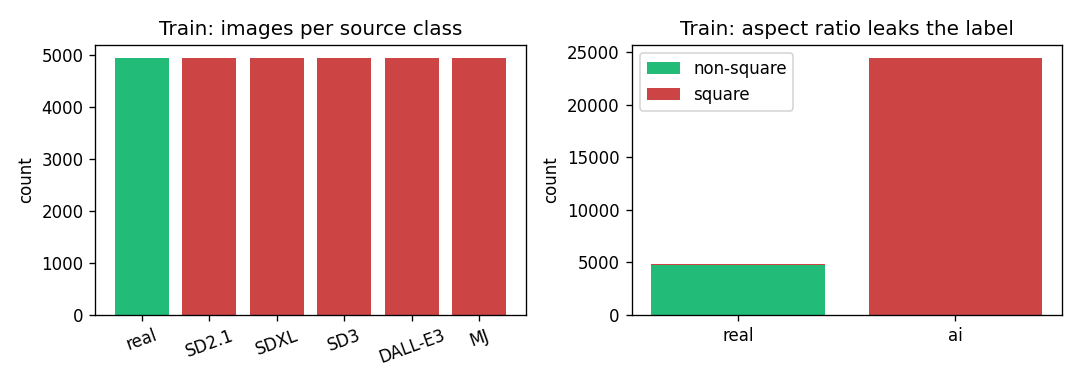
\includegraphics[width=0.84\linewidth]{fig_class_aspect.png}
  \caption{Left: balanced source-class counts in train. Right: in train, real
  images are non-square and AI images are square this is a shortcut absent from the
  $320^2$ evaluation splits.}
  \label{fig:aspect}
\end{figure}

\begin{figure}[t]
  \centering
  \begin{subfigure}{0.47\linewidth}
    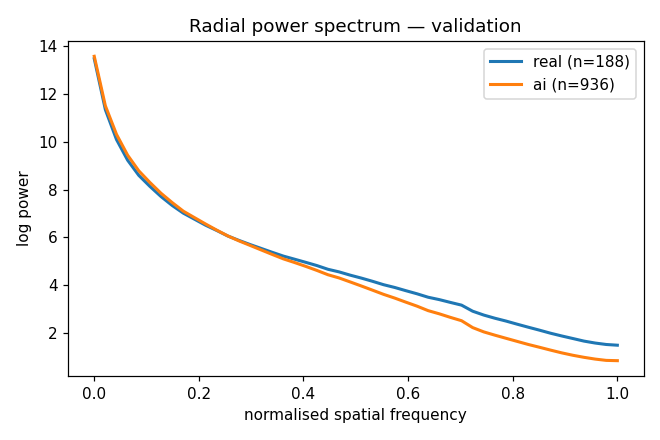
\includegraphics[width=\linewidth]{spectrum_validation.png}
    \caption{Radial power spectrum (validation).}
    \label{fig:spectrum}
  \end{subfigure}\hfill
  \begin{subfigure}{0.39\linewidth}
    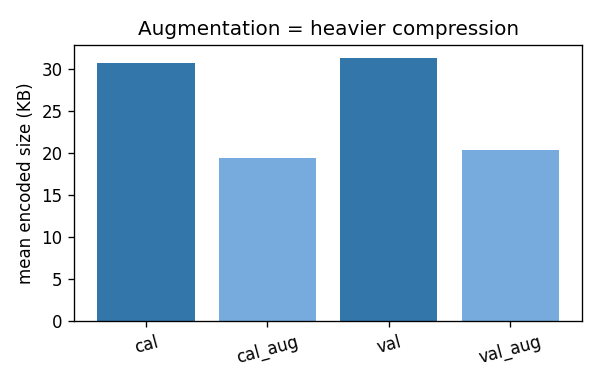
\includegraphics[width=\linewidth]{fig_bytes.png}
    \caption{Encoded size by split.}
    \label{fig:bytes}
  \end{subfigure}
  \caption{Forensic cues. Real images keep more high-frequency energy in the
  radial power spectrum on validation, augmentation compresses images more
  heavily, as shown by encoded size by split.}
\end{figure}
\section{Task 1.2 — Modelling and Tuning under Time Constraints (35\,pts)}
\textbf{Protocol.} We maximise recall on AI images subject to a false-positive
rate (FPR) on real images of at most $20\%$. The operating threshold is
\emph{calibrated automatically} on \texttt{calibration/}: we set it to the
$(1-\tau)$ quantile of the P(AI) scores of real calibration images with a target
$\tau=\Targetfpr$, leaving margin below the $0.20$ limit for the hidden holdout.
The threshold is never hand-set, and \texttt{validation/} is held out purely to
verify the realised FPR.

\textbf{Two model families.} (1) \emph{Classical baseline}: engineered forensic
features — a 32-bin radial FFT spectrum, colour/saturation statistics and
high-pass residual statistics — fed to a histogram gradient-boosted tree. It
trains in seconds and, as Table~\ref{tab:t2} shows, reaches
recall~$\BaseValRecall$ at FPR~$\BaseValFpr$ on validation. Its most important
features (permutation importance) are the highest-frequency spectral bins and
the high-vs-low-frequency contrast, confirming the Task~1.1 analysis
(Fig.~\ref{fig:imp}). (2) \emph{CNN from scratch}: a compact VGG-style network
with a $5{\times}5$ stride-2 stem (so the body runs at half resolution for CPU
speed while the first layer still sees full $\ImgSize$px detail), BatchNorm and
global average pooling ($\approx\!\CnnParams$k parameters). Input is the squared
RGB image at $\ImgSize^2$; inside the network we additionally concatenate a fixed
high-pass residual (RGB minus a $3{\times}3$ blur) as extra channels, giving the
detector an explicit forensic cue motivated by the Task~1.1 spectral analysis
while keeping the external input plain RGB.

\textbf{Efficient, reproducible training.} The Appendix~C reference takes
$\RefSeconds$\,s for 35 steps on our machine; our \texttt{train.py} runs in
$\TrainSeconds$\,s ($\TrainRatio\times$ reference, within the $5\times$
guideline) and well under the 1800\,s timeout. Because CPU speed varies, the
training loop \emph{measures} its own step time and sizes a one-cycle LR
schedule to the number of epochs that fit the budget, so the learning rate
anneals fully regardless of hardware; the best checkpoint (by validation recall
subject to the FPR margin) is flushed whenever it improves, so an early timeout
still yields a usable model. We use class-weighted cross-entropy (real weighted
$\sim\!3\times$) so the minority real class is not ignored.

\textbf{Results and ablations.} Table~\ref{tab:t2} compares both families. The
CNN reaches recall~$\CnnValRecall$ at FPR~$\CnnValFpr$ on validation, meeting
the $0.8$ recall target while keeping the FPR safely below the $0.20$ limit, and
clearly outperforms the classical baseline (recall~$\BaseValRecall$). Key choices that mattered: squaring the inputs (removing the
aspect-ratio shortcut — without it validation FPR collapses), BatchNorm (fast
from-scratch convergence in the few affordable epochs), the stride-2 stem (lets
us keep $\ImgSize$px inputs within budget), and calibrating on a held-out split
(the realised validation FPR tracks the target).

\begin{table}[t]
\centering\small
\begin{tabular}{lcccc}
\toprule
 & \multicolumn{2}{c}{validation} & \multicolumn{2}{c}{validation\_augmented}\\
 \cmidrule(lr){2-3}\cmidrule(lr){4-5}
Model & FPR$_\text{real}$ & recall$_\text{AI}$ & FPR$_\text{real}$ & recall$_\text{AI}$\\
\midrule
Classical (features + GBT) & \BaseValFpr & \BaseValRecall & \BaseAugFpr & \BaseAugRecall\\
CNN — Task 2 (clean)       & \CnnValFpr  & \CnnValRecall  & \CnnAugFpr  & \CnnAugRecall\\
CNN — Task 3 (augmented)   & \AugValFpr  & \AugValRecall  & \AugAugFpr  & \AugAugRecall\\
\bottomrule
\end{tabular}
\caption{Operating point (threshold auto-calibrated on \texttt{calibration/} to
keep FPR safely below the $0.20$ limit; Task~2 target $0.15$, Task~3 a more
conservative $0.14$ for the augmented distribution). The constraint holds on
\emph{validation} for every row; the clean models violate it on
\texttt{validation\_augmented} ($0.262$/$0.225$), which is exactly what the
augmented model repairs ($0.107$).}
\label{tab:t2}
\end{table}

\section{Task 1.3 — Data Augmentation and Robustness (30\,pts)}
\textbf{Motivation.} The classical model's FPR jumps to $\BaseAugFpr$ on
\texttt{validation\_augmented} (constraint violated) and the clean CNN also
degrades, because the high-frequency forensic cue is erased by compression,
blur and rescaling. We therefore make the detector robust by \emph{continuing
training from the Task~2 checkpoint} with on-the-fly augmentation.

\textbf{Strategy.} Each batch is randomly perturbed with the transformations the
exercise highlights plus light photometric noise: downscale-then-upscale
(resolution loss), JPEG recompression (quality $30$–$95$), Gaussian blur,
brightness/contrast jitter, additive noise and horizontal flips. This forces the
network onto content/structure cues that survive perturbation rather than fragile
spectral fingerprints. Epochs are selected on a \emph{combined} clean+augmented
validation set (so we do not pick the least-robust early epoch), and the
threshold is recalibrated on the combined clean+augmented calibration real
images at a slightly conservative target ($0.14$) so the FPR constraint holds
under perturbation as well as on clean data despite the noisy small-sample FPR.

\textbf{Results.} Table~\ref{tab:t2} (last row) shows the augmented model lifts
recall on \texttt{validation\_augmented} from $\CnnAugRecall$ (clean CNN) to
$\AugAugRecall$ at FPR~$\AugAugFpr$, clearing the $0.6$ target, while keeping
competitive clean-validation performance (recall~$\AugValRecall$ at
FPR~$\AugValFpr$). Robustness improves substantially at a small clean-accuracy
cost — the expected trade-off.

\section{Task 1.4 — Explainability (20\,pts)}
We analyse the trained CNN with three complementary methods on validation images
(Fig.~\ref{fig:explain}): vanilla-gradient saliency, Grad-CAM on the last
convolutional block, and occlusion sensitivity (sliding a neutral patch and
measuring the drop in P(AI)). We examine the most borderline true-positive (AI),
true-negative (real), false-positive and false-negative cases.

\textbf{Findings.} Saliency is noisy and spatially \emph{distributed} rather than
tied to one object, and Grad-CAM frequently highlights broad background/sky
regions instead of the main subject — consistent with a detector that keys on
global texture statistics rather than semantics. The occlusion analysis is the
most revealing: replacing a patch with neutral grey almost always \emph{raises}
P(AI) (negative $\Delta$P(AI) in Fig.~\ref{fig:explain}), i.e.\ the model reads
flat, low-detail regions as AI-like. Averaged over many images
(Fig.~\ref{fig:occ}) this effect is strongest in the image centre (mean
$\Delta$P(AI) centre vs.\ border $\OccCenterReal$ vs.\ $\OccBorderReal$ for real,
$\OccCenterAi$ vs.\ $\OccBorderAi$ for AI), exposing two biases worth flagging: a
\emph{smoothness confound} (AI images are smoother, so the model equates
smoothness with ``fake'') and a mild \emph{centre bias}. These also explain the
errors: \emph{false positives} are smooth, low-detail real photos, and
\emph{false negatives} are unusually detailed AI images. We therefore treat the
explanations critically — the model relies on a genuine but shortcut-prone cue
(local detail/smoothness) rather than a single robust artefact, which is exactly
why the Task~1.3 augmentation (which perturbs detail and compression) is needed.

\begin{figure}[t]
  \centering
  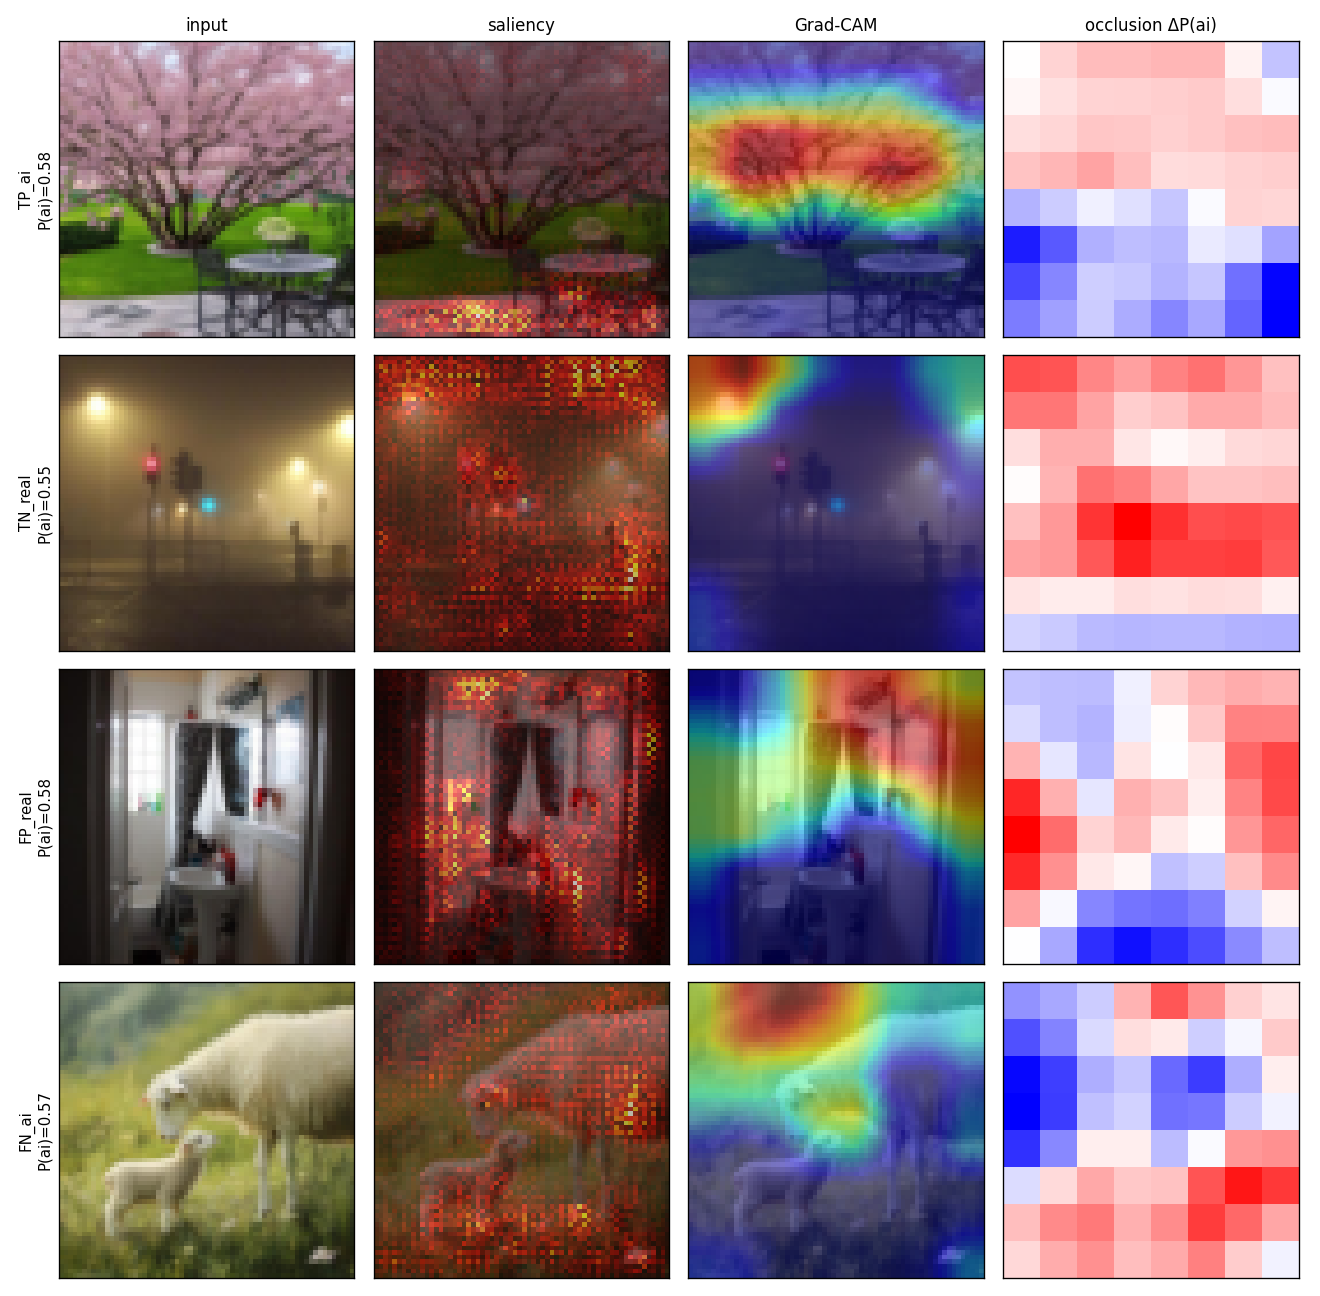
\includegraphics[width=0.86\linewidth]{explain_examples.png}
  \caption{Per-case explanations (rows: borderline TP-AI, TN-real, FP, FN).
  Columns: input, saliency, Grad-CAM, occlusion $\Delta$P(AI).}
  \label{fig:explain}
\end{figure}
\begin{figure}[t]
  \centering
  \begin{subfigure}{0.4\linewidth}
    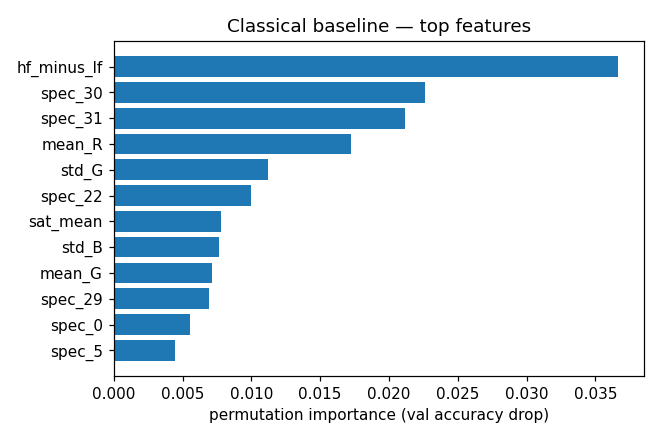
\includegraphics[width=\linewidth]{baseline_importance.png}
    \caption{Classical feature importance.}\label{fig:imp}
  \end{subfigure}\hfill
  \begin{subfigure}{0.52\linewidth}
    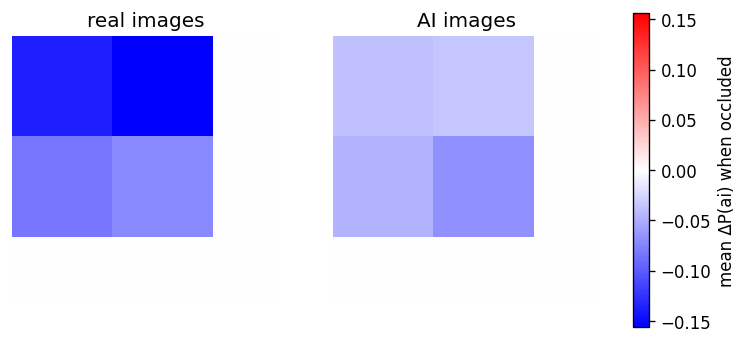
\includegraphics[width=\linewidth]{explain_occlusion_avg.png}
    \caption{Mean occlusion importance (real vs.\ AI).}\label{fig:occ}
  \end{subfigure}
  \caption{What the models rely on: high-frequency spectral bins (a) and a mild
  centre bias in spatial attention (b).}
\end{figure}

\section{Reproducibility and Conclusion}
The solution is fully containerised (CPU-only \texttt{torch}, no runtime
downloads), deterministic (fixed seeds, capped threads) and respects the
read-only data mount by writing all artefacts under \texttt{artifacts/}. We
identified and neutralised an aspect-ratio shortcut, met the Task~2 target
(recall~$\CnnValRecall$ at FPR~$\CnnValFpr\le0.20$), and improved robustness to
recall~$\AugAugRecall$ on augmented data within the same CPU budget. The main
remaining risks are the small number of real calibration/validation images
(noisy FPR estimates, mitigated by the calibration margin) and the residual
centring/smoothness biases surfaced by the explainability analysis.

\end{document}
